\deu{\section{Datenanalyse}\index{Datenanalyse}}
\eng{\section{Data analysis}\index{Data analysis}}
\setcounter{aufgabenNummer}{1}
  \renewcommand{\kAufgabenBuchstabe}{D}




\subsection{Vorbemerkungen}
\paragraph{Abkürzungen}

$n$ = Anzahl Werte

$Q_1$ = erstes Quartil

$IQR$ = Interquartilsrange = Quartilsdifferenz (QD) = $Q_3 - Q_1$

$\varsigma$ = Standardabweichung (Nenner $n$).

$\overline{x}$ = empirischer Mittelwert

$med$ = Median

$Q_3$ = drittes Quartil

$R$ = Range = Spannweite

\subsection{Grundlagen}

\begin{enumerate}
\item Das Säulendiagramm zeigt die Anzahl Kinder pro Familie in einer Siedlung mit
$n=150$ Familien (10 Familien haben keine Kinder, 25 Familien haben 1
  Kind, ...).

\makebox{\includegraphics[width=10cm]{img/stoch/statistic_anz_familien_anz_kinder.png}}

a) Berechnen Sie die relativen Häufigkeiten als Dezimalzahl (3
Dezimalen) und in Prozenten (1 Dezimale).

b) Berechnen Sie die durchschnittliche Kinderzahl pro Familie

c) Erklären Sie anhand dieses Beispiels die Begriffe

\textit{Stichprobenumfang\index{Stichprobe}\index{Stichprobenumfang}, Merkmalsträger\index{Merkmalsträger}, Merkmal\index{Merkmal}, Merkmalsprägung\index{Merkmalsprägung},
  absolute Häufigkeit\index{absolute
    Häufigkeit}\index{Häufigkeit!absolute}, relative
  Häufigkeit\index{relative Häufigkeit}\index{Häufigkeit!relative}}

d) Wie viele Kinder leben in dieser Siedlung?

\item

  Gegeben sind folgende Rohdaten:

  7, 5, 3, 8, 1, 2, 10, 5, 8, 9, 2

  \begin{enumerate}[label=\alph*)]
  \item Erstellen Sie eine geordnete Liste.
  \item Auf welchem Rang\index{Rang} befindet sich der Wert 3?
    \item Welcher Wert befindet sich auf dem mittleren Rang?
  \end{enumerate}

  \subsubsection{}

  
\end{enumerate}


\subsection{Datenerhebung: Problematik von Ausreißern}

\begin{enumerate}
\item Das Durchschnittsvermögen in einer kleinen Gemeine mit 250
  steuerpflichtigen Personen betrug CHF 175\,600.-.

  Durch den Zuzug einer einzigen vermögenden Person erhöhte sich
  dieser Durchschnitt auf CHF 220\,900.-. Wie hoch ist das Vermögen
  dieser Person?

\item Das monatliche Durchschnittseinkommen in einer Firma mit 850
  Beschäftigten beträgt CHF 7\,250.-. Die drei Spitzenverdiener dieser
  Firma verdienen monatlich je CHF 86\,000.-.
  Berechnen Sie das monatliche Durchschnittseinkommen, wenn diese drei
  Spitzenwerte nicht berücksichtigt werden.

\item
  In einer Schulklasse ergaben sich bei der Auswertung einer Prüfung
  folgende Punktezahlen:

  35, 58, 59, 4, 38, 43, 45, 52, 49, 55

  a) Berechnen Sie Mittelwert und Median.

  b) Berechnen sie den Mittelwert ohne den Ausreißer 4.

\item
  10 Eier haben folgende Gewichte in Gramm:

  52.8, 55.9, 58.2, 57.1, 60.4, 69.1 57.9, 58.0, 62.5, 65.0

  Nun wird aus Jux zu den Eiern ein Gips-Ei hinzugelegt. Dadurch
  erhöht sich das Durchschnittsgewicht um 3.48 Gramm pro Ei.

  Berechnen Sie das Gewicht des Gips-Eies.

  Runden Sie auf 0.1 Gramm genau.
  
\end{enumerate}


\subsection{Diagramme (Säulendiagramm, Histogramm, Boxplot)}

\begin{enumerate}
\item \textbf{Säulendiagramm}

  In einer Ausstellung wurden im Laufe einer Woche folgende
  Besucherzahlen ermittelt:

  \begin{tabular}{lllllll}
    Montag & Dienstag & Mittwoch & Donnerstag & Freitag & Samstag & Sonntag \\
    350    & 321      & 647      & 519        & 844     & 1\,314  & 2\,522
  \end{tabular}

  Zeichnen Sie ein \textbf{Säulendiagramm} mit den relativen
  Häufigkeiten in \%.

\item \textbf{Säulendiagramm und Boxplot}

  Hier sehen Sie die Prüfungspunkte in einer Klasse.

  1) Urliste:

  76, 74, 82, 96, 66, 76, 78, 72, 52, 86, 84, 76, 78, 92, 82, 74, 88,
  62

  2) Hier sehen Sie die selben Zahlen geordnet:

  52, 62, 66, 72, 74, 74, 76, 76, 76, 78, 78, 82, 82, 84, 86, 88, 92, 96

  \begin{enumerate}[label=\alph*)]
  \item
    Teilen Sie die Daten in Klassen ein: [50; 60), [60; 70), usw.
        \textit{(Klassenbreite = 10 Punkte).} Zeichnen Sie ein
        Säulendiagramm mit den relativen Häufigkeiten. Zeichnen Sie
        die Säulen aneinanderstossend.

      \item
        Zeichnen Sie einen \textbf{Boxplot}.
      \item
        Bestimmen Sie den \textbf{Mittelwert}.
      \item
        Bestimmen sie den \textbf{Modalwert} (Modus).
      \item
        Bestimmen Sie die \textbf{Quartilsdifferenz} \textit{IQR}.
    \end{enumerate}

\item \textbf{Klassendiagramm, Säulendiagramm, Boxplot}
 Die Messung der Körpergrösse von 100 18-jährigen Schülern liefert
 folgende Zahlen:

 \begin{tabular}{lcccccccccc}
   Grösse in cm & 163 & 164 & 165 & 166 & 167 & 168 & 169 & 170 & 171 & 172\\
   Anzahl      &  1  &  1  &  1  &  3  &  3  &  3  &  4  &  6  &  5  &  5
   \end{tabular}

 \begin{tabular}{lcccccccccc}
   Grösse in cm & 173 & 174 & 175 & 176 & 177 & 178 & 179 & 180 & 181 & 182\\
   Anzahl      &  4  &  7  &  6  &  5  &  5  &  7  &  5  &  4  &  4  &  6
   \end{tabular}

  \begin{tabular}{lcccccc}
   Grösse in cm & 183 & 184 & 185 & 186 & 187 & 188\\
   Anzahl      &  5  &  3  &  3  &  2  &  1  &  1 
  \end{tabular}

  \begin{enumerate}[label=\alph*)]
  \item Erstellen Sie eine Klasseneinteilung mit Klassenbreite 5cm:

    Klasse 1: [160cm; 165cm)

      Klasse 2: [165cm; 170cm)

        usw.

        Zeichnen Sie anschliessend ein Säulendiagramm mit den relativen
        Häufigkeiten in Prozent. Zeichnen Sie die Säulen
        aneinanderstossend.

        \item Zeichnen Sie einen Boxplot mit diesen Daten.
\end{enumerate}


\item \textbf{Vergleich zweier Boxplots}

  Wurfweiten beim Ballwurf in Metern:

  Versuchsreihe 1:

  34.0, 34.4, 32.2, 33.5, 35.2, 32.9, 32.6, 34.3, 33.2, 34.1,
  33.2, 33.2, 34.0, 32.7. 34.8, 33.5, 33.5

  Versuchsreihe 2:

  32.8, 33.7, 34,9, 34.3, 34.6, 32.3, 34.0, 33.9, 33.0, 32.4,
  31.1, 35.5, 31.7, 34.8, 33.5, 32.4

  Erstellen Sie für beide Versuchsreihen je einen Boxplot (Darstellung
  mit gleicher Skala, sodass ein Vergleich möglich wird).



  \item{Informationen aus einem Diagramm herauslesen}

    Praliné-Kugeln in einer Packung; Darstellung der absoluten
    Häufigkeiten:
    
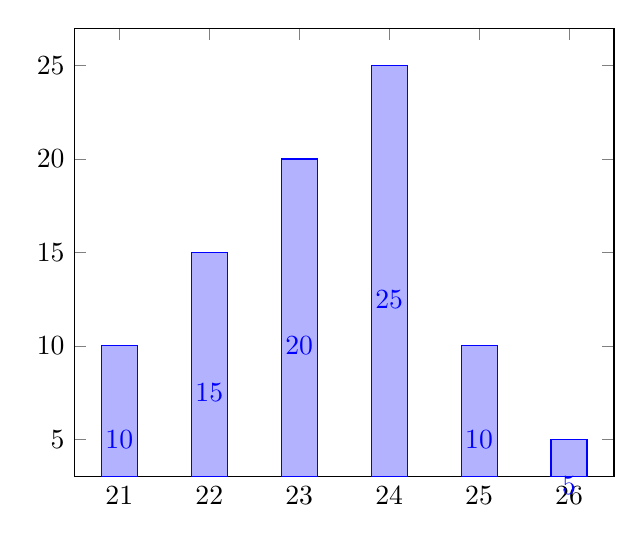
\begin{tikzpicture}\begin{axis}[ybar stacked,nodes near coords,bar
      width=0.4,]\addplot
    coordinates{(21,10) (22,15) (23, 20) (24, 25) (25, 10) (26, 5)};\end{axis}\end{tikzpicture}

Bestimmen Sie Mittelwert, Median und Standardabweichung.
Rechnen Sie mit den Klassenmitteln.

\end{enumerate}


\subsection{Masszahlen (Mittelwert, Media, Quartile,
  Standardabweichung, Quartilsdifferenz)}

\textit{Einige Lehrplanziele dieses Kapitels wurden bereits in den
  vorhergehenden Aufgaben behandelt: Geordnete Liste, Klassenbildung,
  Mittelwert (mit Ausreisser-Problematik), Median, Standardabweichung,
  Quartilsdifferenz.}

\begin{enumerate}
\item In einer Klasse wurden folgende 18 Prüfungsnoten erzielt:

  \begin{tabular}{llllllllll}
    3 & 3 & 3.5 & 3.5 & 4   & 4 & 4.5 & 4.5 & 4.5 & 4.5\\
    5 & 5 & 5.5 & 5.5 & 5.5 & 6 & 6   & 6
  \end{tabular}

  Berechnen Sie \textbf{Mittelwert} und \textbf{Standardabweichung}
  mit Hilfe des Rechners.

\item Drei \textbf{Streumasse}: \textbf{Spannweite R (Range)},
  \textbf{Quartilsdifferenz IQR}, \textbf{Standardabweichung $\sigma$}

  Gegeben sind folgende Daten, die bereits geordnet sind:

  \begin{tabular}{llllllllll}
    2.5 & 2.8 & 3.2 & 3.5 & 3.5 & 4.1 & 4.2 & 4.7 & 4.8 & 4.8\\
    5.4 & 5.5 & 6
  \end{tabular}

  Ermitteln Sie die \textbf{Spannweite (Range)}, die
  \textbf{Quartilsdifferenz} und die \textbf{Standardabweichung} (auf
  2 Dezimalen genau).
  
  
  \end{enumerate}


\newpage
